\documentclass{book}
\setcounter{tocdepth}{1}
\title{A Consumer-Centric Approach to RESTful API Design\newline{}REVIEW COPY DO NOT DISTRIBUTE}
\author{Thomas Hunter II}
\date{January 2014}
\usepackage{graphicx}
\usepackage{hyperref}
\begin{document}

\maketitle

\tableofcontents

\newpage

\chapter{Introduction}

An API represents a contract between data/business logic located on your Server and Consumers who wish to interact with your data. Breaking this contract will result in angry emails from developers and sad sad users with broken mobile apps. Designing a hard-to-use API will result in few or no Third-Party Consumers. On the other hand, building a great API and adhering to this contract will result in substantially more Third-Party Consumers and can elevate your service from a closed-source product to an open platform.

Building an API is one of the most important things you can do to increase the value of your service. By having an API, your service / core application has the potential to become a platform from which other services grow. Look at the current huge tech companies: Facebook, Twitter, Google, GitHub, Amazon, Netflix... None of them would be nearly as big as they are today if they hadn't opened up their data via API. In fact, an entire industry exists with the sole purpose of consuming data provided by said platforms.

The easier your API is to consume, the more people that will consume it.

The principles of this document, if followed while designing and operating your API, will ensure that Consumers will grok your API while substantially reducing support tickets. Developers will travel from tech conference to tech conference telling everyone what a pleasure working with your API is and convincing them to sign up.

\section{Approach}

This book will take a language-agnostic approach to showing you good API design. While there will be a few code examples here and there, you won't actually need to run any of them to understand what is going on. In fact, this book would make a good candidate for sitting on the back of your toilet.

Code examples will often be done in a couple different languages, e.g. PHP and Node.js.

A lot of this is philosophical, not so much technical.

\section{Intended Audience}

Anyone who has built a few websites, knows how to serve up a webpage over HTTP in their platform of choice. Knowing how to read and write HTTP headers is also important. Knowing generic SQL syntax is useful as well, as some example queries are shown in many sections.

\section{Goals of this Book}

By the time you're done reading this book you'll have a high-level understanding of how to build a great RESTful API Ecosystem. This book will not cover the technical details of how to write code an API from scratch.


\chapter{Data Design and Abstraction}

Interacting with data using a REST API is all about boiling down all of the intricate business logic and data storage your service provides into the four basic CRUD concepts (\emph{Create}, \emph{Read}, \emph{Update}, \emph{Delete}). Your application may have all sorts of complex actions such as sending a text message or resizing an image or moving a file, but if you do enough planning and abstraction, everything can be represented as CRUD.

Planning how your API will look begins earlier than you'd think; first you need to decide how your data will be designed and how your core service / application will work. If you're doing \href{http://blog.pop.co/post/67465239611/why-we-chose-api-first-development}{API First Development} this should be easy. If you're attaching an API to an existing project, you may need to provide more abstraction.

Occasionally, a Collection can represent a database table, and a Resource can represent a row within that table. However, this is not the usual case. In fact, your API should abstract away as much of your data and business logic as possible. It is very important that you don't overwhelm Third-Party Developers with any complex application data, if you do they won't want to use your API.

There are also many parts of your service which you SHOULD NOT expose via API at all. A common example is that many APIs will not allow third parties to create users.

Sometimes multiple tables should be represented as a single resource. Maybe even one table having multiple resources, if it makes sense (although, you may have made some poor database design decisions).

\section {Abstraction Examples}

For both the good and bad abstraction example, we'll make use of the same fictional service. Pretend that you control a web service which sends messages to different users and messages can either be sent as a text message or an email, depending on the preferences for a particular user.

Don't worry too much about the technical parts of the examples; we'll get to them in a later chapter. For now, just think of them as simple function calls with inputs and outputs.

\subsection{An Example of Bad Abstraction}

This example will include numerous shortcomings.

\subsubsection{Getting User Preference}

\begin{verbatim}
GET /get_user_preferences/12

{
  "notification_preference": 1
}
\end{verbatim}

This first API Endpoint is called \texttt{get\_user\_preference}, and is called by passing in the ID of the user whose preference we are looking for. The name of and Endpoint should just be a simple noun (or pair of nouns if need be). You should never add the action being performed (in this case \texttt{get}). The reason one should use a simple noun is that it tells you exactly what the following ID value represents. Does the \texttt{12} shown below represent user \texttt{12}? Or some user preference \texttt{12} concept which might not correlate 1:1 the same as users?

Another problem with this example is the response contains the integer \texttt{1}. Internally to the service, there is a fictional set of constants, where \texttt{1} refers to sending a text, and \texttt{2} refers to sending an email. Even if this value is written in the API documentation, a Consumer of the API is not going to remember the value, and every time they look it up they'll be annoyed and lose productivity.

Another problem is that there's an API Endpoint dedicated specifically to getting a user preference. Something like this should have been merged with another endpoint for getting all the data about a particular user.

\subsubsection{Sending a Text or Email (Two Endpoints)}

\begin{verbatim}
POST /users/12/send_text
POST /users/12/send_email

{
  "message": "Hello World",
  "sent": "2013-01-06 21:02:00"
}
\end{verbatim}

This second and third endpoints have the same problem as the previous endpoint wherein the action is part of the URL (in this case \texttt{send}). These endpoints don't represent data, as the previous one did, they specifically represent an action. Building APIs with these sorts of endpoints is very common.

Another issue with this is that the business logic for determining which method of notification is used is left to the Consumer to take care of! Sure, the Consumer can make a request to get the user preference for sending messages, but what if they ignore it? You're going to have some very annoyed users.

Whenever you find yourself creating two endpoints with the exact same expected request inputs and response outputs, there may be an issue with abstraction and the two might be better off combines.

Also, there is no way to refer to previous instances of sending notifications to a user. Sure, the Consumer could record this information somewhere in a database, but it would be beneficial if the API made available a method for looking up previous notifications.

\subsection{An Example of Good Abstraction}

With the same messaging web service, here's a cleaner, RESTful method for sending messages to users.

\subsubsection{Creating a Notification}

\begin{verbatim}
POST /notifications

{
  "user_id": 12,
  "message": "Hello World"
}

{
  "id": 1000,
  "user_id": 12,
  "message": "Hello World",
  "medium": "email",
  "created": "2013-01-06 21:02:00"
}
\end{verbatim}

In this example, only a single endpoint is needed for doing the same work as the previous three endpoints of the bad example. The first JSON document is the request and the second is the response. This endpoint is simply called \texttt{notifications}, and as a Consumer you are working with creating notification objects.

When the Consumer wants to notify a user, they are actually creating a new notification object, thereby abstracting the concept of performing an action to the concept of creating an object. Of course, an action can't be undone or changed, so the Consumer can't DELETE or PUT a notification object.

Another important concept with this example is that the business logic of determining which method for contacting a user is abstracted away from the Consumer entirely, hence the lack of an endpoint for getting the users notificaiton preference.

In the example response, we do have a medium attribute which represents the notification method, but that can be hidden entirely depending on if your Consumers would ever need to know it (perhaps their application has a dashboard which mentions the last time a text/email was sent, and the verbage should be correct).

\chapter{Raw HTTP Packet}

Since everything we do is over HTTP, let's look at a dissection of an HTTP packet. It's surprising how many developers who have been building websites for years don't know what an HTTP packet looks like! When the Consumer sends a Request to the Server, they provide a set of Key/Value pairs, called a Header, along with two newline characters, and finally the request body. This is all sent in the same packet.

The server then responds in the say Key/Value pair format, with two newlines and then the response body. HTTP is very much a request/response protocol; there is no "Push" support (the Server sending data to the Consumer unprovoked), unless you use a different protocol such as Websockets.

\section{Example HTTP Request}

\begin{verbatim}
POST /v1/animal HTTP/1.1
Host: api.example.org
Accept: application/json
Content-Type: application/json
Content-Length: 24

{
  "name": "Gir",
  "animal_type": 12
}
\end{verbatim}

\section{Example HTTP Response}

\begin{verbatim}
HTTP/1.1 200 OK
Date: Wed, 18 Dec 2013 06:08:22 GMT
Content-Type: application/json
Access-Control-Max-Age: 1728000
Cache-Control: no-cache

{
  "id": 12,
  "created": 1386363036,
  "modified": 1386363036,
  "name": "Gir",
  "animal_type": 12
}
\end{verbatim}

\section{Debugging HTTP Traffic}

When designing your API, you should be able to work with tools which allow you to look at raw HTTP packets. Consider using \href{https://www.wireshark.org}{Wireshark}, for example. Also, make sure you are using a framework / web server which allows you to read and change as many of these fields as possible.

Here's an example of a heavier HTTP request of a form submission on a website. Notice all of the data sent back and forth using HTTP headers.

\begin{figure}[ht!]
\centering
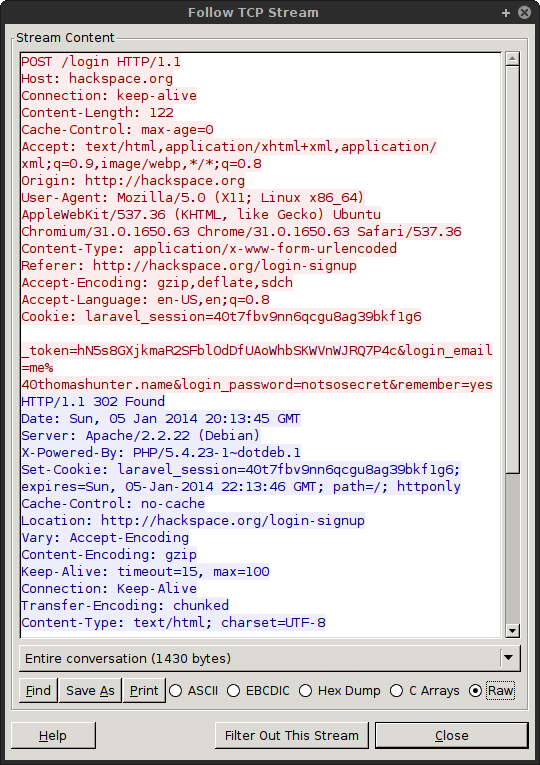
\includegraphics[height=90mm]{images/wireshark.png}
\caption{Wireshark Screenshot}
\label{overflow}
\end{figure}


\chapter{API Root URL}

The root location of your API is important, believe it or not. When a developer (read as code archaeologist) inherits an old project using your API and needs to build new features, they may not know about your service at all. Perhaps all they know is a list of URLs which the Consumer calls out to. It's important that the root entry point into your API is as simple as possible, as a long complex URL will appear daunting and can turn developers away.

\section{Root URL Location}

Here are two common URL Root Locations:

\begin{itemize}
\item \texttt{https://example.org/api/*}
\item \texttt{https://api.example.com/*}
\end{itemize}

If your application is huge, or you anticipate it becoming huge, putting the API on its own subdomain (e.g. \textbf{api.}) is a good choice. This can allow for some more flexible scalability down the road. It can also be useful for preventing which cookie data can be shared between the content website and the API.

If you anticipate your API will never grow to be that large, or you want a much simpler application setup (e.g. you want to host the website AND API from the same framework), placing your API beneath a URL segment at the root of the domain (e.g. \textbf{/api/}) works as well.

Also, notice the HTTPS prefix. As a good RESTful API, you MUST host your API behind HTTPS.

Don't use a different TLD (Top Level Domain) for hosting your API than you do for hosting your website. This may sound tempting, as your main domain could be \textbf{example.com}, and your API and developer documentation be entirely located on \textbf{example.io}. However, there is no logical relationship between these two domains and an adversary could have purchased \textbf{example.io} and is posing as a legitamate counterpart to \textbf{example.com}. Also, the "code archeologist" might only have knowledge of one domain and not the other. Finally, if you \emph{do} want to share some cookies between the two websites (e.g. an authenticated user on \textbf{example.com} can be automatically logged into the developer site) it cannot be done as easily with two separate TLDs than with a subdomain or subdirectory.

\section{Content at the Root}

It's a good idea to have content at the root of your API. Hitting the root of GitHub's API returns a listing of endpoints, for example. Personally, I'm a fan of having the root URL give information which a lost developer would find useful, e.g., how to get to the developer documentation for the API.

Here's a truncated example of the content provided by the \href{https://api.github.com/}{GitHub API Root URL}. Notice how it's both easily readable by a human and easily parsable by a machine.

\begin{verbatim}
{
  "current_user_url": "https://api.github.com/user",
  "authorizations_url": "https://api.github.com/authorizations",
  "emails_url": "https://api.github.com/user/emails",
  ...
}
\end{verbatim}


\chapter{API Versioning}

No matter what you are building, no matter how much planning you do beforehand, your core application is going to change, your data relationships will change, attributes will invariably be added and removed from your Resources. This is just how software development works, and is especially true if your project is alive and used by many people (which is likely the case if you're building an API).

\begin{verbatim}
https://api.example.org/v1/*
\end{verbatim}

Remember than an API is a published contract between a Server and a Consumer. If you make changes to the Servers API and these changes break backwards compatibility, you will break things for your Consumer and they will resent you for it. Do it enough, and they will leave. To ensure your application evolves AND you keep your Consumers happy, you need to occasionally introduce new versions of the API while still allowing old versions to be accessible.

As a side note, if you are simply ADDING new features to your API, such as new attributes on a Resource (which are not required and the Resource will function without), or if you are ADDING new Endpoints, you do not need to increment your API version number since these changes do not break backwards compatibility. You will want to update your API Documentation (your Contract), of course.

Over time you can deprecate old versions of the API. To deprecate a feature doesn't mean to shut if off or diminish the quality of it, but to tell Consumers of your API that the older version will be removed on a specific date and that they should upgrade to a newer version.

\begin{verbatim}
Accept: application/json+v1;
\end{verbatim}

A good RESTful API will keep track of the version in the URL. The other most common solution is to put a version number in a request header, but after working with many different Third Party Developers, I can tell you that adding headers is no where near as easy as adding a URL Segment.


\chapter{HTTP Verbs}

Surely you know about GET and POST requests. These are the two most commonly requests used when your browser visits different webpages. All browsers, such as IE6, have been able to make these two requests. TODO Wording

There are four and a half very important HTTP verbs that you need to know about. I say "and a half", because the PATCH verb is very similar to the PUT verb, and two two are often combined by many an API developer. Here are the verbs, and next to them are their associated database call (I'm assuming most people reading this know more about writing to a database than designing an API).

\begin{itemize}
\item \textbf{GET}
    \begin{itemize}
    \item Retrieve a specific Resource from the Server
    \item Retrieve a listing of Resources from the Server
    \item Think of this as a SQL SELECT statement
    \end{itemize}
\item \textbf{POST}
    \begin{itemize}
    \item Creates a new Resource on the Server
    \item Think of this as a SQL INSERT statement
    \end{itemize}
\item \textbf{PUT}
    \begin{itemize}
    \item Update a Resource on the Server
    \item Provide the entire Resource
    \item Think of the SQL UPDATE statement providing null values for some keys
    \end{itemize}
\item \textbf{PATCH}
    \begin{itemize}
    \item Update a Resource on the Server
    \item Provide only changed attributes
    \item Like the SQL UPDATE statement providing only a few keys
    \end{itemize}
\item \textbf{DELETE}
    \begin{itemize}
    \item Remove a Resource from the Server
    \item Similar to the SQL DELETE statement
    \end{itemize}
\end{itemize}

Here are two lesser known HTTP verbs. Feel free to use them in your API, but they aren't 100% necessary.

\begin{itemize}
\item \textbf{HEAD}
    \begin{itemize}
    \item Retrieve meta data about a Resource
    \item Such as a hash of the data or when it was last updated
    \end{itemize}
\item \textbf{OPTIONS}
    \begin{itemize}
    \item Retrieve information about what the Consumer is allowed to do with the Resource
    \end{itemize}
\end{itemize}

A good RESTful API will make use of the four and a half HTTP verbs for allowing third parties to interact with its data, and will never include actions / verbs as URL segments.

Typically, GET requests can be cached (and often are!) Browsers, for example, will cache GET requests (depending on cache headers), and will go as far as prompt the user if they attempt to POST for a second time. A HEAD request is basically a GET without the response body, and can be cached as well.


\chapter{URL Endpoints}

An Endpoint is a URL within your API which points to a specific Resource or a Collection of Resources.

Honestly, it doesn't matter too much if the endpoints are singular or plural. What does matter is that you stay consistent. The examples in this book are plural.

If you were building a fictional API to represent several different Zoo's, each containing many Animals (with an animal belonging to exactly one Zoo), employees (who can work at multiple zoos) and keeping track of the species of each animal, you might have the following endpoints:

\begin{itemize}
\item \texttt{https://api.example.com/v1/\textbf{zoos}}
\item \texttt{https://api.example.com/v1/\textbf{animals}}
\item \texttt{https://api.example.com/v1/\textbf{animal\_types}}
\item \texttt{https://api.example.com/v1/\textbf{employees}}
\end{itemize}

Each piece of data separated by slashes is a URL Segment. Try to keep these as simple as possible.

When referring to what each endpoint can do, you'll want to list valid HTTP Verb and Endpoint combinations. For example, here's a semi-comprehensive list of actions one can perform with our fictional API. Notice that I've preceded each endpoint with the HTTP Verb, as this is the same notation used within an HTTP Request header.

\begin{itemize}
\item \texttt{GET /zoos}: List all Zoos (ID and Name, not too much detail)
\item \texttt{POST /zoos}: Create a new Zoo
\item \texttt{GET /zoos/ZID}: Retrieve an entire Zoo object
\item \texttt{PUT /zoos/ZID}: Update a Zoo (entire object)
\item \texttt{PATCH /zoos/ZID}: Update a Zoo (partial object)
\item \texttt{DELETE /zoos/ZID}: Delete a Zoo
\item \texttt{GET /zoos/ZID/animals}: Retrieve a listing of Animals (ID and Name).
\item \texttt{GET /animals}: List all Animals (ID and Name).
\item \texttt{POST /animals}: Create a new Animal
\item \texttt{GET /animals/AID}: Retrieve an Animal object
\item \texttt{PUT /animals/AID}: Update an Animal (entire object)
\item \texttt{PATCH /animals/AID}: Update an Animal (partial object)
\item \texttt{GET /animal\_types}: Retrieve a listing (ID and Name) of all Animal Types
\item \texttt{GET /animal\_types/ATID}: Retrieve an entire Animal Type object
\item \texttt{GET /employees}: Retrieve an entire list of Employees
\item \texttt{GET /employees/EID}: Retreive a specific Employee
\item \texttt{GET /zoos/ZID/employees}: Retrieve a listing of Employees at this Zoo
\item \texttt{POST /employees}: Create a new Employee
\item \texttt{POST /zoos/ZID/employees}: Hire an Employee at a specific Zoo
\item \texttt{DELETE /zoos/ZID/employees/EID}: Fire an Employee from a specific Zoo
\end{itemize}

In the above list, ZID means Zoo ID, AID means Animal ID, EID means Employee ID, and ATID means Animal Type ID. Having a key in your documentation for whatever convention you choose is a good idea.

I've left out the common API URL prefix in the above examples for brevity. While this can be fine during communications, in your actual API documentation, you should always display the full URL to each endpoint (e.g. GET http://api.example.com/v1/animal\_type/ATID).

Notice how the relationships between data is displayed, specifically the many to many relationships between employees and zoos. By adding an additional URL segment, one can perform more specific interactions. Of course there is no HTTP verb for "FIRE"-ing an employee, but by performing a DELETE on an Employee located within a Zoo, we're able to achieve the same effect.


\chapter{Resource Filtering}

When a Consumer makes a GET request for a Collection, it is important that you give them a list of every single object matching the requested criteria. This list could be massive. But, it is important that you don't perform any arbitrary limitations of the data. It is these arbitrary limits which make it hard for a third party developer to know what is going on. If they request a certain Collection, and iterate over the results, and they never see more than 100 items, it is now their job to figure out where this limit is imposed. Is their ORM buggy and limiting items to 100? Is the network chopping up large packets?

Minimize arbitrary limits imposed on Third Party Developers.

You do want to offer the ability for a Consumer to specify some sort of filtering/limitation of the results. The most important reason for this, as far as the Consumer is concerned, is that the network payload is minimal and the Consumer gets their results back as soon as possible. Another reason for this is the Consumer may be lazy, and if the Server can do filtering and pagination for them, all the better. The not-so-important reason (from the Consumers perspective), yet a great benefit for the Server, is that the request will be less resource intensive.

Filtering is mostly useful for performing GETs on Collections of resources. Since these are GET requests, filtering information should be passed via the URL. Here are some examples of the types of filtering you could conceivably add to your API:

\begin{itemize}
\item \texttt{?limit=10\&offset=20}: Pagination of results (\texttt{LIMIT 20, 10})
\item \texttt{?animal\_type\_id=1}: Filter records which match the following condition (\texttt{WHERE animal\_type\_id = 1})
\item \texttt{?sort\_attribute=name,asc}: Sort the results based on the specified attribute (\texttt{ORDER BY name ASC})
\end{itemize}

Some of these filterings can be redundant with endpoint URLS. In the Endpoints chapter we mentioned \texttt{GET /zoo/ZID/animals}. This would be the same thing as \texttt{GET /animals?zoo\_id=ZID}. Dedicated endpoints being made available to the Consumer will make their lives easier, this is especially true with requests you anticipate they will make a lot. In the documentation, mention this redundancy so that Third Party Developers aren't left wondering if differences exist.

Also, this goes without saying, but whenever you perform filtering or sorting of data, make sure you white-list the columns for which the Consumer can filter and sort by. We don't want any database errors being sent to Consumers!


\chapter{Respone Attribute Filtering}

Often times, when a Consumer is making a GET request to a specific Resource or Collection of Resources, they do not care about all of the attributes belonging to the resource. Having so much data could be a network bottleneck. Responding with less data can also reduce the overhead on your server, for example it may prevent an unneccesary database \texttt{JOIN}.

Again, since we're dealing with GET requests, you'll want to accept a URL parameter for whitelisting parameters. In theory, blacklisting could work as well, but as new attributes appear in Resources over time (since additions are backwards compatible) the Consumer ends up receiving data it doesn't want.

The parameter name you choose isn't too important. It could be "filter" or the overly-verbose "attribute\_whitelist". Consistency between different Endpoints is what is most important.

\section{Example Unfiltered Single-Resource Request}

In this example request, the default representation of a user object includes data from two tables joined together. One of the tables is the obvious user table, and another table contains some textual data related to a user called user\_descriptions.

\subsection{Request URL}

\begin{verbatim}
GET http://api.example.org/user/12
\end{verbatim}

\subsection{Resulting SQL Query}

\begin{verbatim}
SELECT * FROM user LEFT JOIN user_desc ON user.id = user_desc.id
  WHERE user.id = 12;
\end{verbatim}

\subsection{Response Body}

\begin{verbatim}
{
  "id": 12,
  "name": "Thomas Hunter II",
  "age": 27,
  "email": "me@thomashunter.name",
  "description": "Blah blah blah blah blah."
}
\end{verbatim}

\section{Example Filtered Single-Resource Request}

In this next example, the consumer has requested a filtered list of attributes. So, we're returning less data. If you make use of an ORM, filtering of this data should be pretty simple, however if you're manually writing SQL queries, more effort may be involved.

\subsection{Request URL}

\begin{verbatim}
GET http://api.example.org/user/12?whitelist=id,name,email
\end{verbatim}

\subsection{Resulting SQL Query}

\begin{verbatim}
SELECT id, name, email FROM user WHERE user.id = 12;
\end{verbatim}

\subsection{Response Body}

\begin{verbatim}
{
  "id": 12,
  "name": "Thomas Hunter II",
  "email": "me@thomashunter.name"
}
\end{verbatim}


\chapter{JSON Request Body}

There are two common ways a Web Browser will send data to a Web Server. If you're using a common web language/framwork for building an API, such as PHP or Express.js or Ruby on Rails, you're already consuming data using these two methods. Web Servers (e.g. Apache or NGINX) abstract the differences of these two methods and will usually work with your programming language to provide data in one easy to consume format. The two methods are called Multipart Form Data (required for file uploads), as well as Form URL Encoded.

Below you'll see examples of both of those methods just so that you understand how the browser and server usually upload data. Unfortunately, neither of them are adaquate for sending complex data to a RESTful server. The third example is the method you should be accepting data as.

\section{Example Form URL Encoded Request}

This method is used by Websites for accepting simple data forms from a web browser.

\begin{verbatim}
POST /login HTTP/1.1
Host: example.com
Content-Length: 31
Accept: text/html
Content-Type: application/x-www-form-urlencoded

username=root&password=Zion0101
\end{verbatim}

\section{Example Multipart Form Data Request}

This method is used by Websites for accepting more complex data from a web browser, such as file uploads.

\begin{verbatim}
POST /file_upload HTTP/1.1
Host: example.com
Content-Length: 275
Accept: text/html
Content-Type: multipart/form-data; boundary=----RANDOM_jDMUxq4Ot5

------RANDOM_jDMUxq4Ot5
Content-Disposition: form-data; name="file"; filename="hello.txt"
Content-Type: application/octet-stream

Hello World
------RANDOM_jDMUxq4Ot5
Content-Disposition: form-data; name="some_checkbox"

on
------RANDOM_jDMUxq4Ot5--
\end{verbatim}

\section{Example JSON Request}

This method is much better for uploading data. The JSON document used for the Request can be very similar to the JSON document used for the Response. JSON can specify the type of data (e.g. Integers, Strings, Booleans), while also allowing for hierarchal relationships of data.

\begin{verbatim}
POST /v1/animal HTTP/1.1
Host: api.example.org
Accept: application/json
Content-Type: application/json
Content-Length: 24

{
  "name": "Gir",
  "animal_type": 12
}
\end{verbatim}


\chapter{HTTP Response Status Codes}

It is very important that as a RESTful API, you make use of the proper HTTP Status Codes; they are a standard after all! Various network equipment is able to read these status codes, e.g. load balancers can be configured to avoid sending requests to a web server sending out lots of 50x errors. Client libraries know if a request has succeeded or failed depending on the Status Code. There are a plethora of \href{http://www.w3.org/Protocols/rfc2616/rfc2616-sec10.html}{HTTP Status Codes} to choose from, however this list should be a good starting point:

\begin{itemize}
\item \texttt{\textbf{200} OK}
    \begin{itemize}
    \item GET Requests
    \item The Consumer requested data from the Server, and the Server found it for them (Idempotent)
    \end{itemize}
\item \texttt{\textbf{201} ACCEPTED}
    \begin{itemize}
    \item POST / PUT / PATCH Requests
    \item The Consumer gave the Server data, and the Server accepted it
    \end{itemize}
\item \texttt{\textbf{202} NO CONTENT}
    \begin{itemize}
    \item DELETE Requests
    \item The Consumer asked the Server to delete a Resource, and the Server deleted it
    \end{itemize}
\item \texttt{\textbf{400} INVALID REQUEST}
    \begin{itemize}
    \item POST / PUT / PATCH Requests
    \item The Consumer gave bad data to the Server, and the Server did nothing with it (Idempotent)
    \end{itemize}
\item \texttt{\textbf{404} NOT FOUND}
    \begin{itemize}
    \item All Requests
    \item The Consumer referenced an inexistant Resource or Collection, and the Server did nothing (Idempotent)
    \end{itemize}
\item \texttt{\textbf{500} INTERNAL SERVER ERROR}
    \begin{itemize}
    \item All Requests
    \item The Server encountered an error, and the Consumer has no knowledge if the request was successful
    \end{itemize}
\end{itemize}

\section{Status Code Ranges}

The \textbf{1xx} range is reserved for low-level HTTP stuff, and you'll very likely go your entire career without manually sending one of these status codes.

The \textbf{2xx} range is reserved for successful messages where all goes as planned. Do your best to ensure your Server sends as many of these to the Consumer as possible.

The \textbf{3xx} range is reserved for traffic redirection. Most APIs do not use these requests much (not nearly as often as the SEO folks use them ;), however, the newer Hypermedia style APIs will make more use of these.

The \textbf{4xx} range is reserved for responding to errors made by the Consumer, e.g. they're providing bad data or asking for things which don't exist. These requests should be be idempotent, and not change the state of the server.

The \textbf{5xx} range is reserved as a response when the Server makes a mistake. Often times, these errors are thrown by low-level functions even outside of the developers hands, to ensure a Consumer gets some sort of response. The Consumer can't possibly know the state of the server when a 5xx response is received, and so these should be avoidable.


\chapter{Response Content Types}

Currently, the most "exciting" of APIs provide JSON data from RESTful interfaces. This includes Facebook, Twitter, GitHub, you name it. XML appears to have lost the war a while ago (except in large corporate environments). SOAP, thankfully, is all but dead, and we really don't see much APIs providing HTML to be consumed (unless, that is, you're building a scraper!)

Here's a Google Trends graph comparing the terms JSON API, XML API, and SOAP API, which should give a good feel for how their popularity has changed over time:

\begin{figure}[ht!]
\centering
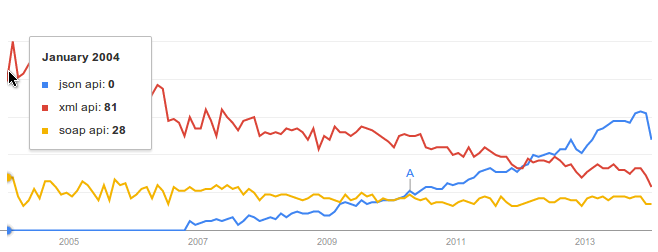
\includegraphics[width=110mm]{images/xml-vs-json-vs-soap-google-trends.png}
\caption{Google Trends for JSON API, XML API, and SOAP API}
\label{overflow}
\end{figure}

Developers using popular languages and frameworks can very likely parse any valid data format you return to them. You can even provide data in any of the aforementioned data formats (not including SOAP) quite easily, if you're building a common response object and using a different serializer. What does matter though, is that you make use of the Accept header when responding with data.

Some API creators recommend adding a .json, .xml, or .html file extension to the URL (after the endpoint) for specifying the content type to be returned. With the different extensions added, we've now got different URLs for the same Resources. Use the Accept header, which is built into the HTTP spec for this purpose, and if you can't provide data in a format the Consumer wants, reply with a \texttt{406 Not Acceptable} response.


\chapter{Expected Response Bodies}

When a Consumer makes a request to the Server, something needs to be returned in the response. Depending on the HTTP Verb being used, the response will be different. Here's a good list to adhere to:

\begin{itemize}
\item \texttt{GET /collection}
    \begin{itemize}
    \item Return a listing (array) of Resource objects
    \end{itemize}
\item \texttt{GET /collection/resource\_id}
    \begin{itemize}
    \item Return a singular Resource object
    \end{itemize}
\item \texttt{POST /collection}
    \begin{itemize}
    \item Return the newly created Resource object
    \end{itemize}
\item \texttt{PUT /collection/resource\_id}
    \begin{itemize}
    \item Return the complete Resource object
    \end{itemize}
\item \texttt{PATCH /collection/resource\_id}
    \begin{itemize}
    \item Return the complete Resource object
    \end{itemize}
\item \texttt{DELETE /collection/resource\_id}
    \begin{itemize}
    \item Return an empty document
    \end{itemize}
\end{itemize}

Note that when a Consumer creates a Resource, they usually do not know the ID of the Resource being created (nor other attributes such as created and modified timestamps, if applicable). These additional attributes are returned with the resulting Response, which is vital for the Consumer to keep track of things.


\chapter{Response Document Standards}

When responding with a document representing a Collection, it is usually adaquate to return a top-level array containing each Resource object. Likewise, when responding with a document representing a Resource, simply returning a top-level object containing the Resource is good-enough.

However, there are some standards people have developed for encapsulating these items in a standardized envelope to help give the Consumer some context when parsing the responses.

For example, if making a filtered request limiting the Collection to containing only 10 Resources, how do you let the Consumer know how many total records exist? If an error occurs, sure you reply with a 4XX or 5XX HTTP Status Code, but what about an object in the body representing an error? These different response document standards provide a standardized method for returning this meta data.

\section{JSON Schema}

\href{http://json-schema.org/}{json-schema.org}

TODO

\section{JSON API}

\href{http://jsonapi.org/}{jsonapi.org}

TODO

\section{Siren}

\href{http://sirenspec.org}{sirenspec.org}

TODO


\chapter{Authentication}

There are two common paradigms your server may represent. In the three legged paradigm, a third-party API consumer is making requests on behalf of a user of your website / service. In a two-legged paradigm, there really isn't a user involved.

\section{Two Legged Authentication}

TODO: Something proprietary? Simple GET parameter?

TODO: Research solutions

\section{Three Legged Authentication}

TODO: Mention things need to be revoked.

Typically, a Server will want to know exactly who is making which Requests. Some APIs provide endpoints to be consumed by the general (anonymous) public, but most of the time work is being perform on behalf of someone.

\href{https://tools.ietf.org/html/rfc6749}{OAuth 2.0} provides a great way of doing this. With each Request, you can be sure you know which Consumer is making requests, which User they are making requests on behalf of, and provides a (mostly) standardized way of expiring access or allowing Users to revoke access from a Consumer, all without the need for a third-party consumer to know the Users login credentials.

There are also \href{http://tools.ietf.org/html/rfc5849}{OAuth 1.0} and \href{https://dev.twitter.com/docs/oauth/xauth}{xAuth}, which fill the same space. Whichever method you choose, make sure it is something common and well documented with many different libraries written for the languages/platforms which your Consumers will likely be using.

I can honestly tell you that OAuth 1.0a, while it is the most secure of the options, is a huge pain in the ass to implement. I was surprised by the number of Third Party Developers who had to implement their own library since one didn't exist for their language already. I've spent enough hours debugging cryptic "invalid signature" errors to recommend you choose an alternative.


\chapter{API Permissions}

This is mostly applicable with Three Legged Authentication.

\begin{figure}[ht!]
\centering
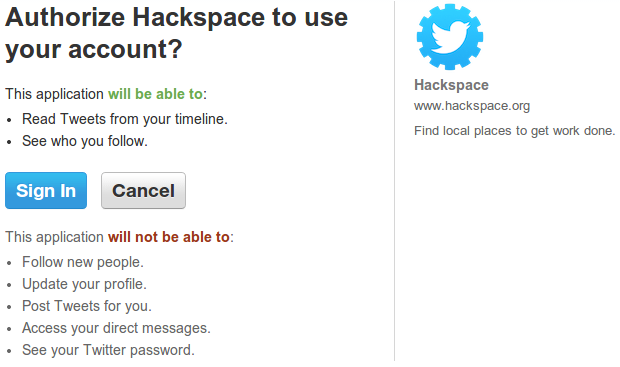
\includegraphics[width=90mm]{images/permissions-twitter.png}
\caption{Twitter OAuth Permissions}
\label{overflow}
\end{figure}


\chapter{API Analytics}

Keep track of the version/endpoints of your API being used by Consumers. This can be as simple as incrementing an integer in a database each time a request is made. There are many reasons that keeping track of API Analytics is a good idea, for example, the most commonly used API calls should be made efficient.

For the purposes of building an API which Third Party Developers will love, the most important thing is that when you do deprecate a version of your API, you can actually contact developers using deprecated API features. This is the perfect way to remind them to upgrade before you kill the old API version.

The process of Third Party Developer notification can be automated, e.g. mail the developer every time 10,000 requests to a deprecated feature are made.


\chapter{Writing good Documentation}

Honestly, if you don't conform 100\% to the criteria in this guide, your API will not necessarily be horrible. However, if you don't properly document your API, nobody is going to know how to use it, and it WILL be a horrible API.

Make your Documentation available to unauthenticated developers.

Do not use automatic documentation generators, or if you do, at least make sure you're doctoring it up and making it presentable.

Do not truncate example request and response bodies; show the whole thing. Use a syntax highlighter in your documentation.

Document expected response codes and possible error messages for each endpoint, and what could have gone wrong to cause those error messages.

If you've got the spare time, build a developer API console so that developers can immediately experiment with your API. It's not as hard as you might think and developers (both internal and third party) will love you for it!

Make sure your documentation can be printed; CSS is a powerful thing; don't be afraid to hide that sidebar when the docs are printed. Even if nobody ever prints a physical copy, you'd be surprised at how many developers like to print to PDF for offline reading.


\chapter{Developer Console}

Building a Developer Console will allow developers to quickly test API commands without having to run their applications over and over. If commands can be linked to from within the documentation, this is even better.

\begin{figure}[ht!]
\centering
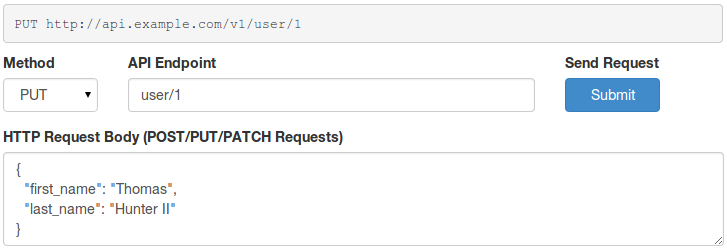
\includegraphics[width=110mm]{images/api-console.png}
\caption{Example API Console}
\label{overflow}
\end{figure}


\chapter{Hypermedia APIs: REST Evolved}

Hypermedia APIs are very likely the future of RESTful API design. They're actually a pretty amazing concept, going "back to the roots" of how HTTP and HTML was intended to work.

When working with non-Hypermedia RESTful APIs, the URL Endpoints are part of the contract between the Server and the Consumer. These Endpoints MUST be known by the Consumer ahead of time, and changing them means the Consumer is no longer able to communicate with the Server as intended. This, as you can assume, is quite a limitation.

Now, API Consumers are of course not the only user agent making HTTP requests on the Internet. Far from it. Humans, with their web browsers, are the most common user agent making HTTP requests. Humans, however, are NOT locked into this predefined Endpoint URL contract that RESTful APIs are. What makes humans so special? Well, they're able to read content, click links for headings which look interesting, and in general explore a website and interpret content to get to where they want to go. If a URL changes, a human is not affected (unless, that is, they bookmarked a page, in which case they go to the homepage and find a new route to their beloved data).

The Hypermedia API concept works the same way a human would. Requesting the Root of the API returns a listing of URLs which point perhaps to each collection of information, and describing each collection in a way which the Consumer can understand. Providing IDs for each resource isn't important (or necessarily required), as long as a URL is provided.

With the Consumer of a Hypermedia API crawling links and gathering information, URLs are always up-to-date within responses, and do not need to be known beforehand as part of a contract. If a URL is ever cached, and a subsequent request returns a 404, the Consumer can simply go back to the root and discover the content again.

When retrieving a list of Resources within a Collection, an attribute containing a complete URL for the individual Resources are returned. When performing a POST/PATCH/PUT, the response can be a 3xx redirect to the complete Resource.

JSON doesn't quite give us the semantics we need for specifying which attributes are URLs, nor how URLs relate to the current document. HTML, as you can probably guess, does provide this information. We may very well see our APIs coming full circle and returning back to consuming HTML. Considering how far we've come with CSS, one day we may even see  it be common practice for APIs and Websites to use the exact same URLs and content.

Imagine a tool on the internet that you want to use. Could be Google Calendar, or Meetup, or Facebook Events. Now, imagine that you want to use other tools too, like email or instant messenger. Normally, integrations between tools are only convenient if you're dealing with a massive suite of tools, like you see offered by Microsoft or Google. TODO

Now, imagine that these amazing tools by different companies can all work with each other as tightly as these massive suite tools. The best of both worlds. Imagine it automatically working, them automatically discovering each other and configuring themselves to work together nicely. This is a future offered by hypermedia APIs. TODO

\section{ATOM: An Early Hypermedia API}

\begin{verbatim}
<?xml version="1.0" encoding="utf-8"?>
<feed xmlns="http://www.w3.org/2005/Atom">
  <title>Example Feed</title>
  <subtitle>A subtitle.</subtitle>
  <link href="http://example.org/feed/" rel="self" />
  <link href="http://example.org/" />
  <id>urn:uuid:60a76c80-d399-11d9-b91C-0003939e0af6</id>
  <updated>2003-12-13T18:30:02Z</updated>
  <entry>
    <title>Atom-Powered Robots Run Amok</title>
    <link href="http://example.org/2003/12/13/atom03" />
    <link rel="alternate" type="text/html" href="http://example.org/2003/12/13/atom03.html"/>
    <link rel="edit" href="http://example.org/2003/12/13/atom03/edit"/>
    <id>urn:uuid:1225c695-cfb8-4ebb-aaaa-80da344efa6a</id>
    <updated>2003-12-13T18:30:02Z</updated>
    <summary>Some text.</summary>
      <author>
        <name>John Doe</name>
        <email>johndoe@example.com</email>
      </author>
  </entry>
</feed>
\end{verbatim}


\chapter{Alternatives to REST}

\section{JSON RPC}

\href{http://www.jsonrpc.org/specification}{JSON RPC} is a relatively popular alternative to REST for exposing functionality over a network. Whereas REST is required to be used via HTTP, JSON RPC doesn't actually have a protocol requirement. It can be sent over sockets, be used with Inter Process Communication (IPC), and yes, it can function over HTTP.

Unlike REST which requires an abstraction of the Server functionality of business logic and data into simple objects which can be acted upon using CRUD, JSON RPC calls typically map to existing functions within your application.

When a client makes a call using JSON RPC, they specify the name of a function to execute, as well as arguments to the function. Arguments can be in the form of either ordered parameters (using a JSON Array), or named parameters (using a JSON Object).

A big part of the specification is the envelope which the data being sent through adheres to. The concept of a URL doesn't really exist (if you're using JSON RPC over HTTP, there's probably a single URL all requests are sent through, and every request is likely sent as POST requests).

JSON RPC is mostly useful for situations where you don't have an HTTP server, for example multiplayer games or embedded systems. If you already have an HTTP server for your product or service, REST is probably the correct solution.

When dealing with HTTP, every Request and Response is guaranteed to be paired together correctly. Due to the asynchronous nature of sockets and other such communication protocols, requests need to provide a unique ID value, and the corresponding response needs to provide the same ID.

For more information about the JSON RPC Specification visit \href{http://www.jsonrpc.org/specification}{jsonrpc.org}.

\subsection{Example JSON RPC Request}

\begin{verbatim}
{"jsonrpc": "2.0", "method": "subtract", "params": [42, 23],
  "id": 1}
\end{verbatim}

\subsection{Example JSON RPC Response}

\begin{verbatim}
{"jsonrpc": "2.0", "result": 19, "id": 1}
\end{verbatim}


\section{XML SOAP}

This is a sort of example of Hypermedia API's gone wrong. Very complex. Also, nobody likes XML. Mention that I don't know much.

Big in corporate environments.

Mention how it Sucks


\chapter{About the Author and Reviewers}

\section{Author: Thomas Hunter II}

At the time of this writing, \href{http://thomashunter.name}{Thomas Hunter II} works as a Developer Advocate / API Architect with Copy.com, where his number one concern is getting a well-documented API into the hands of Consumers. He also recently co-hosted a talk at the Ann Arbor PHP MySQL meetup on the topic of RESTful API Design.

\section{Reviewer: John Sheehan}

John is an API fanatic with over 15 years of experience working in a wide variety of IT and software development roles. As an early employee at Twilio, John lead the developer evangelism program and worked as a Product Manager for Developer Experience. After Twilio, John was Platform Lead at IFTTT working with API providers to create new channels. John is also the creator of \href{https://www.github.com/restsharp/restsharp}{RestSharp}, \href{http://www.apidigest.com/}{API Digest}, \href{http://www.api-jobs.com/}{API Jobs} and co-host of \href{http://trafficandweather.io/}{Traffic and Weather}, an API and cloud podcast.

\section{Reviewer: Kevin Swiber}

Senior software developer and Enterprise Architect with experience in multiple languages, platforms, and operating systems. Currently focused on cloud-based solutions and scalable, distributed systems. Leading the charge for open source development and inter-platform collaboration in the greater software development community.

\end{document}
